\documentclass{article}
\usepackage[utf8]{inputenc}
\usepackage[french]{babel} 
\usepackage[T1]{fontenc} 


\usepackage{graphicx} 
\usepackage{float} 
\usepackage{hyperref}

\title{Assistance for the Construction of Critical Embedded Control Systems}
\author{Alexis Giraudet \and Asma Khelifi \and Jean-Christophe Guérin \and Geoffrey Desbrosses \and Léo Cassiau \and Tantely Randriamaharavomanana \and Ugo Mahey}


\date{Novembre 2016}

\begin{document}

\maketitle

\tableofcontents

\newpage

\section*{Introduction}
    %Phrase d'accroche
    
    % Objectif perso
    Ce document résume le travail effectué au cours du Capstone project de 2\ieme{} année du master ALMA 2016 - 2017. Ce projet est mené par des étudiants de la faculté des sciences et techniques de Nantes, et le sujet est proposé par M. Attiogbe\footnote{\url{http://pagesperso.lina.univ-nantes.fr/~attiogbe-c/}} et M. André\footnote{\url{http://pagesperso.lina.univ-nantes.fr/~andre-p/}}, tous les deux enseignants-chercheurs à l'université de Nantes.
    
    \bigskip
    
    % Contexte et enjeux
    L'objectif du projet est de réaliser, en équipe, un outil facilitant la rédaction des programmes utilisant la méthode B. La méthode B est une méthode formelle permettant d'assurer le bon fonctionnement des programmes, et notamment dans le cas qui nous intéresse ici, les programmes présents sur les systèmes embarqués. Ces systèmes possèdent des actuateurs et des senseurs, qui permettent de prendre connaissance et d'agir sur l'environnement du système. Ceci nous permet de commencer à décrire le comportement du système, appelé le contrôleur. C'est donc à partir la spécification du système embarqué que l'on commence à rédiger le programme du contrôleur. Notre outil a pour but de faciliter le passage entre la spécification du système et la spécification du contrôleur.
    
    \bigskip
    
    %Problematique
    %- Facile à utiliser, possible de mettre sur le web, partager les données, réut
    Pour programmer notre outil nous avons dû faire des choix sur les différentes techniques à utiliser. Par exemple, il nous a été suggéré que notre outil devait avoir la possibilité d'être déployé sur un serveur Web. Pour cela nous avons décidé d'utiliser J2E, une des spécifications de JAVA. Cette spécification nous permet d'intégrer facilement notre code JAVA (grâce aux servlets) à un serveur (jetty dans notre cas).%jsais pas si vous voulez le mettre mais dire possibilité de l'exposé en service web jpense que ça peut être bien
    Nous avons également décidé de faire une interface graphique web. Cette interface est destinée aux utilisateurs le but étant de faire quelque chose de clair et simple d'utilisation.%explication de l'ihm 
    
    
    \bigskip
    
    %-Il faut délimiter le moment quand notre outil finit et le B commence
    Une des problématiques principales pour ce projet fut la suivante, comment différencier ce que l'on peut automatiser avec notre outil, c'est-à-dire ce que l'on peut deviner à partir des informations fournies par l'utilisateur, de ce que l'utilisateur doit expliciter ultérieurement. Dans notre cas nous nous appuyons sur le langage B. Il existe des outils déjà existant qui permette d'écrire, de vérifier la syntaxe et d'effectuer des transformations sur ce langage. Un des enjeux est de ne pas avoir à réécrire des choses déjà faites (même si dans le futur notre outil doit pouvoir intégrer ces outils, comme par exemple être en mesure de vérifier de façon syntaxique une entrée utilisateur écrite en B).
    %Ecrire le choix de ce que notre outil fait - bien comprendre les besoins utilisateurs
    
    \bigskip
    
    %Plan
    Ce document commence par analyser et résumé le sujet, puis il s'attarde sur les choix d'implémentations que l'on a fait et enfin une conclusion résume notre expérience acquise tout le temps du projet.
    
\section{Analyse}

\subsection{Diagramme de Gantt}
    
    Diagramme représentant le temps passé sur le projet pour chaque élève.
    
    \begin{figure}[ht]
        \centering
        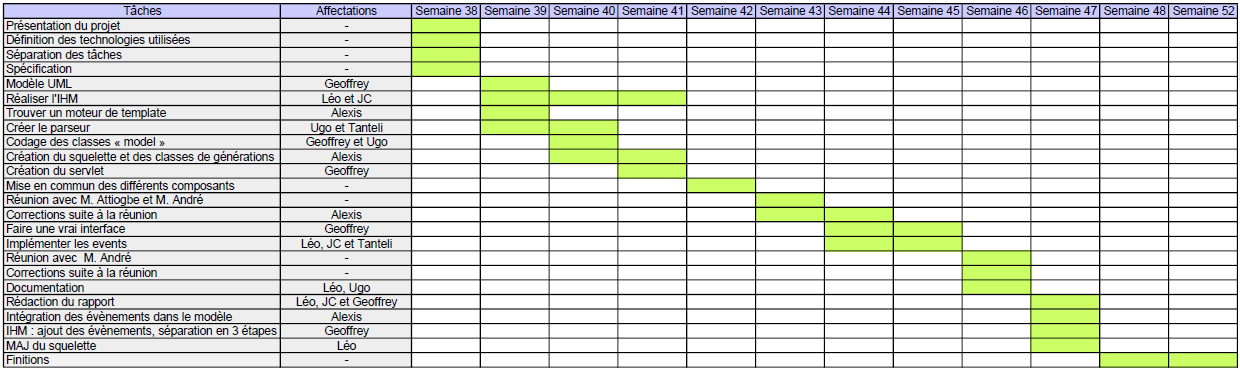
\includegraphics[width=\textwidth]{gantt.png}
        \caption{Diagramme de Gantt}
        \label{fig:gantt}
    \end{figure}
    
%parler de la méthode/démarche qu'il faut implémenter, les étapes...
\subsection{Rapide introduction aux méthodes formelles}

    Les méthodes formelles sont des méthodes permettant de prouver du programme, c'est-à-dire vérifier qu'il ne possède pas de bug. La méthode B est une de ces méthodes, étudié en cours à la faculté des sciences et techniques de Nantes. Ce genre de méthode est particulièrement utilisé dans les systèmes embarqués car ces systèmes restent assez simples pour être prouvé et qu'il est important d'éviter les bugs lors du fonctionnement d'un robot, pour éviter tout comportement dangereux et également car il est plus difficile de corriger un système embarqué.
    
\subsection{Assister la construction des programmes des systèmes embarqués}
    Tout d’abord, notre problème à résoudre avec la méthode B doit correspondre au schéma \ref{fig:ctrl} suivant  : un contrôleur (notre machine) reçoit des informations de l’environnement à l’aide des senseurs, et il agit sur ce même environnement à l’aide d’actuateurs. 
    
    \begin{figure}[ht]
        \centering
        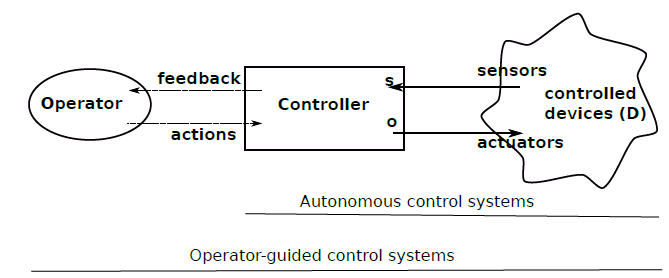
\includegraphics[width=\textwidth]{controller.png}
        \caption{Principe d'un système de contrôle}
        Source : Assistance for the Construction of Critical Embedded Control Systems using Event-B. 2016, Christian Attiogbe (sujet du projet)
        \label{fig:ctrl}
    \end{figure}
    
    Le sujet de notre projet consiste à aider à concevoir le programme du contrôleur (Controller sur la figure \ref{fig:ctrl}). Pour cela, une méthodologie a été proposé avec deux types d'étapes : les étapes dites horizontales et les autres qui sont verticales.
    
\subsubsection{Les étapes horizontales}
    Le processus horizontal correspond à l'étape d'abstraction de l'écriture d'une machine en B, c'est-à-dire l'étape où on l'on définit le comportement du contrôleur tout en prouvant, grâce au prouveur du B, que notre programme est correct. Ce processus possède plusieurs étapes décrient dans le sujet : tout d'abord il est nécessaire de définir la liste des variables. 
    
\paragraph{Liste des variables}
    Il existe quatre catégories de variables, dont on a définit les rôles avec le corps enseignant :
    
        \begin{itemize}
            \item Les variables d'entrées (input) qui correspondent aux valeurs retournés par les senseurs.
            \item Les variables de sorties (output) qui correspondent aux valeurs reçus par les actuateurs.
            \item Les variables de contrôle (control) qui correspondent aux valeurs qui agissent sur l'appareil contrôlé.
            \item Les variables internes (internal) qui correspondent aux valeurs temporaires internes au contrôleur.
        \end{itemize}
        
\paragraph{Les invariants} Ensuite, il faut lister les propriétés du système, qui deviendront les invariants en B. Ce sont donc des propriétés du système qui sont vérifiées à chaque instant, et elles ne sont pas à confondre avec la notion de properties en B.

\paragraph{Les événements} L'étape suivante consiste à générer des événements en fonction des variables précédemment renseignées. Chaque variable d'entrées et de sorties à des événements correspondants (sensing et reaction) qui agissent en lien avec le système contrôlé. Comme chaque système doit avoir des événements de sensing et de reactions, ils sont générés automatiquement.

\subsubsection{Les étapes verticales}
    Les étapes verticales concernent le raffinement de la machine B, ce qui ne concerne pas l'outil que nous avons développé. 
        
\section{Implémentation}
Nous avons décidé de faire ce projet à l'aide du langage JAVA et plus spécifiquement grâce au J2E. C'est ce choix de technologie qui nous est apparu le plus judicieux. En effet notre outil devant être déployé sur un serveur web nous avons choisi la technologie la plus couramment utilisé pour nos besoins. 
%Choix techniques, outils utilisés, pourquoi...

\subsection{Les outils développement}
	Le sujet du projet nous laissait choisir les différentes technologies à manipuler pour réaliser l'outil ACCECS. Cette partie s'attarde sur ces choix et les explique.
    
\subsubsection{Une interface web}
	Après plusieurs discussions avec le corps enseignant, une des premières nécessités était de de rendre l'outil accessible facilement, si possible depuis internet et utilisable par plusieurs usagers en même temps. En effet, l'outil serait amené à être utilisé par des équipes, et les résultats de l'outil doivent être accessibles facilement aux différent membres de l'équipe. Nous avons donc choisi d'utiliser une interface web.
	
	\bigskip
	
	Nous avons choisi d'utiliser bootstrap pour un meilleur rendu en CSS, et car c'est une bibliothèque populaire. Les scripts sont rédigés en simple javascript car c'est une partie assez minime du projet, la plupart des calculs étant fait à l'aide de Java. Enfin, nous avons utilisé Jetty comme serveur par défaut, car il est facile d'utilisation (sous forme de plugin maven).
	
\subsubsection{Le langage utilisée : Java}
    L'essentiel du code est écrit en Java, car c'est le langage sur lequel les membres de l'équipe étaient le plus à l'aise. De plus, grâce aux servlets, il est facile de lier l'interface web et notre code source. Enfin, les de classe de Java permettent de regrouper certaines notions du B. Maven est également utilisé pour gérer facilement les dépendances et faciliter la reprise du projet.

\subsubsection{Le format des données : JSON}
    Nous avons choisi de représenter les données échangées entre l'interface et le code source sous le format JSON, car c'est un format facile à lire et à manipuler, avec des analyseurs syntaxiques disponibles facilement, notamment sur le web. C'est sous ce format que sont enregistrées les données rentrées par l'utilisateur. On peut ainsi enregistrer ces données, créer des jeux de données, les échanger, et les rouvrir sous une autre machine. 

\subsubsection{Le moteur de template Jtwig}
    Les résultats fournis par notre outil se doivent de respecter un squelette correspondant à une machine B. Pour modifier facilement le squelette selon nos besoins, nous avons choisi d'utiliser un moteur de template. Jtwig est l'un d'eux, qui s'avère simple d'utilisation, très complet, compatible avec Java et assez populaire pour espéré qu'il soit maintenu dans les années à venir. 
    
    \subsubsection{Différencier un contrôleur et la future machine B}
    L'un des premiers besoins exprimé par le corps enseignant était que notre outil ne soit pas automatiquement associé à la méthode B. Il doit avant tout servir à spécifier un contrôleur qui va agir sur son environnement. Ce contrôleur possède des actuateurs, des senseurs, etc\dots qui vont servir à définir les premières variables de base. Notre interface doit donc permettre de rentrer ces premières variables ainsi que les premières propriétés déduites uniquement des propriétés du contrôleur, le tout de la manière la plus intuitive celui qui manipule le contrôleur, et non pour celui qui sera amené à rédiger le code en B.
    
\subsubsection{Les évènements}
    Les évènements sont des opérations qui se déclenchent lorsqu'un senseur détecte une valeur critique. On peut déduire des évènements des variables de base indiqués par l'utilisateur, afin de les générer leurs squelettes dans la future machine B. Les variables d'entrées (input) génère ainsi des événements sensoriels (sense) et les variables de sortie (output) génèrent des événements de réactions (reaction). Il existe deux dernières catégories d'événements, ceux de surveillance (monitor) et ceux de contrôles (control). Les événements de contrôles lisent en entrée les variables de contrôles et agissent sur les variables de sortie, tandis que les événements de surveillance lisent les variables d'entrées et agissent sur les variables de contrôles. Il n'est pas possible de générer un squelette pour ces deux types d'événements car les variables de sorties et d'entrées sont impossibles à prévoir.
    
\subsubsection{Les limites liées à la complexité du B}
    La méthode B elle-même s'est avéré être un frein, le but d'ACCECS étant de faciliter le début de la spécification d'une machine B, mais pas d'essayer de remplacer la méthode elle-même. Nous avons donc choisi de ne pas rendre lisible par notre outil du code en B. Cela demanderait de recoder toutes les notions de B en java pour un résultat sûrement de qualité moindre, et un suivi serait nécessaire en fonction des mises à jour du B. Cela représente un travail imposant pour un résultat moindre, car il est vrai que notre outil facilite la maintenance du code B, mais il se veut rester basique.
%\section{Démonstration}
    
\section*{Conclusion}
    Finalement, la réalisation de cet outil nous aura appris à être à l'écoute des besoins du client, ici le corps enseignant, afin de répondre au mieux à leurs attentes. Comprendre leurs exigences demande de non seulement cerner leurs besoins, mais également de comprendre l'aspect technique sans quoi on ne peut pas comprendre les attentes. Ce projet nous aura aussi appris à travailler dans une plus grosse équipe que dans les projets habituels. 

    \bigskip

    Quant à ACCECS, il sera amené à être repris par de futurs étudiants afin de l'améliorer, toujours dans le but d'aider les enseignants dans la conception de contrôleurs. En guise d'amélioration, plusieurs pistes sont envisageables comme l'amélioration de l'ergonomie en fonction des besoins des utilisateurs, le chargement des machines B ou la possibilité de modifier, mais surtout de développer un plugin Eclipse pour intégrer l'outil dans Rodin.

\end{document}
